\chapter{Environment Infrastructure}
\section{Foraging}
\subsection{Inputs, Outputs and Functions}

Foraging has been implemented in the code base. It determines the method of foraging. In short, it is either deer hunting being payoff focused or fishing being a risk averse method of foraging. Deer hunting is linked to a population model, based on a logistics population model. The high level inputs include island IDs, resource contributions from those islands and the chosen foraging method. The high level output is a foraging report which include forage type, input resources, number of participants, number caught, total utility, catch sizes, turn.\newline

A list of useful and important functions can be found on Table \ref{tab:Foraging Main Functions}, together with a description of what they're doing, as well as their inputs and outputs.

\newpage
\begin{table}[!htb]
\begin{center}
\begin{tabular}{|c|c|l|l|l|}
\hline
\textbf{File}                                                                          & \textbf{Functions}                                                                    & \multicolumn{1}{c|}{\textbf{Description}}                                                                                                                                                                               & \multicolumn{1}{c|}{\textbf{Inputs}}                                                                                                                           & \multicolumn{1}{c|}{\textbf{Outputs}}                                                                                                                                           \\ \hline
\multirow{4}{*}{\texttt{deerhunt.go}}                                                  & \texttt{TotalInput}                                                                   & \begin{tabular}[c]{@{}l@{}}Sums the total \\ group resources \\ input of hunt \\ participants\end{tabular}                                                                                                              & \begin{tabular}[c]{@{}l@{}}- Island ID\\ - Foraging \\ Resources\end{tabular}                                                                                  & \begin{tabular}[c]{@{}l@{}}- Total Island \\ Foraging \\ Resources\\ Contributions\end{tabular}                                                                                 \\ \cline{2-5} 
                                                                                       & \texttt{Hunt}                                                                         & \begin{tabular}[c]{@{}l@{}}Returns the \\ utility form a \\ deer hunt and \\ updates population\end{tabular}                                                                                                            & \begin{tabular}[c]{@{}l@{}}- Deer hunt \\ configuration\\ (Max deer per hunt,\\ incremental input \\ Decay,\\  input scaler)\\ - Deer Population\end{tabular}  & \begin{tabular}[c]{@{}l@{}}- Decision of Deer \\ Forage\\ - Participant \\ Resource \\ Contributions\\ - Utility \\ (Cumulative sum \\ of the \\ 'weight of deer')\end{tabular} \\ \cline{2-5} 
                                                                                       & \texttt{DeerReturn}                                                                   & \begin{tabular}[c]{@{}l@{}}Combining two \\ random variables \\ D-Bernoulli random \\ variable (binary \\ probability of \\ catching deer) and \\ W - Continuous \\ random variable\\ (Weight of deer)\end{tabular}     & \begin{tabular}[c]{@{}l@{}}- Deer hunt \\ parameters \\ (Bernoulli variable \\ and exponential \\ variable for weight)\end{tabular}                            & \begin{tabular}[c]{@{}l@{}}- Tier \\ (according to \\ input resources)\end{tabular}                                                                                             \\ \cline{2-5} 
                                                                                       & \texttt{\begin{tabular}[c]{@{}c@{}}getPopulation\\ LinkedProbability\end{tabular}}    & \begin{tabular}[c]{@{}l@{}}Returns the \\ probability\\ of catching a deer \\ with the current \\ running deer \\ population\end{tabular}                                                                               & \begin{tabular}[c]{@{}l@{}}- Deer hunt \\ configuration \\ (Max deer per hunt,\\ incremental input \\ Decay, \\ input scalar)\\ - Deer population\end{tabular} & \begin{tabular}[c]{@{}l@{}}- Bernoulli \\ probability of \\ catching a deer \\ given the current \\ running deer \\ population.\end{tabular}                                    \\ \hline
\multirow{2}{*}{\texttt{\begin{tabular}[c]{@{}c@{}}deer\\ population.go\end{tabular}}} & \texttt{\begin{tabular}[c]{@{}c@{}}createBasic\\ DeerPopulation\\ Model\end{tabular}} & \begin{tabular}[c]{@{}l@{}}Returns a basic \\ population\\  model based on \\ $dP/dt = k(N-y)$ \\ model.\\ $k$ = growth coeff., \\ $N$ = max deer \\ (constants).\end{tabular}                                          & \begin{tabular}[c]{@{}l@{}}- Deer hunt \\ configuration\\ - Logger\end{tabular}                                                                                & \begin{tabular}[c]{@{}l@{}}- Deer Population \\ Model\end{tabular}                                                                                                              \\ \cline{2-5} 
                                                                                       & \texttt{Simulate}                                                                     & \begin{tabular}[c]{@{}l@{}}Simulates the \\ reaction of a deer \\ population over \\ the length of the \\ input to the function \\ (in days) where \\ 0 to a max number \\ of deer are hunted \\ each day.\end{tabular} & \begin{tabular}[c]{@{}l@{}}- Deer \\ Consumption\end{tabular}                                                                                                  & \begin{tabular}[c]{@{}l@{}}- Population \\ Model\end{tabular}                                                                                                                   \\ \hline
\end{tabular}
\end{center}
\end{table}

\newpage
\begin{table}[!htb]
\begin{center}
\begin{tabular}{|c|c|l|l|l|}
\hline
\textbf{File}                        & \textbf{Functions}                                                            & \multicolumn{1}{c|}{\textbf{Description}}                                                                                                                         & \multicolumn{1}{c|}{\textbf{Inputs}}                                                                                                                        & \multicolumn{1}{c|}{\textbf{Outputs}}                                                                                                                                       \\ \hline
\multirow{3}{*}{\texttt{fishing.go}} & \texttt{TotalInput}                                                           & \begin{tabular}[c]{@{}l@{}}Sums the total \\ group resource \\ input of hunt \\ participants.\end{tabular}                                                        & \begin{tabular}[c]{@{}l@{}}- Island ID\\ - Foraging \\ Resources\end{tabular}                                                                               & \begin{tabular}[c]{@{}l@{}}-Total Island \\ Foraging \\ Resource \\ Contributions\end{tabular}                                                                              \\ \cline{2-5} 
                                     & \texttt{fishingReturn}                                                        & \begin{tabular}[c]{@{}l@{}}Returns a \\ random resource\\ amount from a \\ declared normal \\ distribution with \\ an inputted mean \\ and variance.\end{tabular} & \begin{tabular}[c]{@{}l@{}}- Fishing \\ parameters \\ (Mean - mu \\ and \\ Variance - Sigma)\end{tabular}                                                   & \begin{tabular}[c]{@{}l@{}}- Returns \\ the Tier for fish \\ foraging\end{tabular}                                                                                          \\ \cline{2-5} 
                                     & \texttt{Fish}                                                                 & \begin{tabular}[c]{@{}l@{}}Computes the return\\ from a fishing \\ expedition\end{tabular}                                                                        & \begin{tabular}[c]{@{}l@{}}- Fish hunt \\ configuration \\ (Max fish per hunt,\\ incremental input \\ Decay, input scalar \\ - Deer population\end{tabular} & \begin{tabular}[c]{@{}l@{}}- Decision of Fish\\  Forage \\ - Participant \\ Resource \\ Contributions\\ -Utility (cumulative \\ sum of the \\ "size of fish'')\end{tabular} \\ \hline
\multirow{4}{*}{\texttt{helpers.go}} & \texttt{getTotalInput}                                                        & \begin{tabular}[c]{@{}l@{}}Computes the total\\ agent contributions\\ for foraging\end{tabular}                                                                   & \begin{tabular}[c]{@{}l@{}}- Island \\ Contributions\end{tabular}                                                                                           & \begin{tabular}[c]{@{}l@{}}- Total Contributions \\ for Foraging\end{tabular}                                                                                               \\ \cline{2-5} 
                                     & \texttt{\begin{tabular}[c]{@{}c@{}}compile Foraging\\ Report\end{tabular}}     & \begin{tabular}[c]{@{}l@{}}It compiles a \\ foraging\\  report for the given\\ inputs i.e. a \\ summary\\  of foraging activity\end{tabular}                      & \begin{tabular}[c]{@{}l@{}}- Forage type\\ - Island \\ Contributions\\ - Forage Returns\end{tabular}                                                        & - Foraging report                                                                                                                                                           \\ \cline{2-5} 
                                     & \texttt{utilityTier}                                                          & \begin{tabular}[c]{@{}l@{}}Gets the discrete \\ utility tier (i.e. max \\ number of deer/fish) \\ for given scalar \\ resource input.\end{tabular}                & \begin{tabular}[c]{@{}l@{}}- Input Resource\\  Contributions \\ - Max number of \\ deer/fish per hunt\\ - Input scalar\end{tabular}                         & - Discrete utility tier                                                                                                                                                     \\ \cline{2-5} 
                                     & \texttt{Display}                                                              & \begin{tabular}[c]{@{}l@{}}Returns a JSON \\ string for a \\ foraging report\end{tabular}                                                                         & - Foraging Report                                                                                                                                           & - JSON String                                                                                                                                                               \\ \hline
\multirow{3}{*}{\texttt{setup.go}}   & \texttt{CreateDeerHunt}                                                       & \begin{tabular}[c]{@{}l@{}}Receives hunt \\ participants and \\ their contributions \\ and returns a \\ DeerHunt\end{tabular}                                     & \begin{tabular}[c]{@{}l@{}}- Deer hunt \\ configuration \\ - Logger\end{tabular}                                                                            & \begin{tabular}[c]{@{}l@{}}- Deer hunt\\ - Error\end{tabular}                                                                                                               \\ \cline{2-5} 
                                     & \texttt{\begin{tabular}[c]{@{}c@{}}CreateFishing\\ Expedition\end{tabular}}   & \begin{tabular}[c]{@{}l@{}}Receives hunt \\ participants and \\ their contributions \\ and returns a \\ FishHunt\end{tabular}                                     & \begin{tabular}[c]{@{}l@{}}- Island IDs with\\ their contributions\\ - Fish hunt \\ configuration \\ - Logger\end{tabular}                                  & \begin{tabular}[c]{@{}l@{}}- Fishing \\ Expedition\\ - Error\end{tabular}                                                                                                   \\ \cline{2-5} 
                                     & \texttt{\begin{tabular}[c]{@{}c@{}}CreateDeer\\ PopulationModel\end{tabular}} & \begin{tabular}[c]{@{}l@{}}Returns the target\\ population model.\end{tabular}                                                                                    & \begin{tabular}[c]{@{}l@{}}- Deer hunt \\ configuration\\ - Logger\end{tabular}                                                                             & - Population model                                                                                                                                                          \\ \hline
\end{tabular}
\end{center}
\caption{Foraging Main Functions}
\label{tab:Foraging Main Functions}
\end{table}

\newpage
\subsection{Important Implementation Remarks}
\subsubsection{Dynamics of a Collective Hunt}

A deer hunt is modelled as a stochastic process where the expected utility is proportional to the input resources provided for the hunt. There is no limit to the number of teams $m$ that can join a hunt, however, there is a limit to the number of deer $n$ that can be hunted in a single foraging round. Importantly, $n$ should be chosen such that $n < max(m) = 6$, so that, beyond a certain number of hunters, the utility per team decreases as the same expected return could be achieved with less hunters. 

The utility distribution is modelled as being agnostic to the number of hunters; it only depends on the collective amount of resources invested in the hunt. Furthermore, assume the minimum resources to hunt a single deer is $\theta$ and employ the assumption that hunting one deer is independent to another. If we let $\theta=1$\footnote{it is desirable to use 1 in this definition to allow for later scaling by an arbitrary constant to ensure a scale that is commensurate with other resource-based quantities in the environment} and define the expected return for a single deer as $E[U]=\mu$, for a given real-valued collective resource input $x$ (across all hunt participants), the expected total utility $U_{\theta}$ is proposed as follows:

\begin{equation}
U_{\theta}=\left\{\begin{array}{ll}
\mu & x \in[\Delta^0; \ \Delta^1)\\
2 \mu & x\in[\Delta^1; \ \Delta^2)\\
3 \mu & x\in[\Delta^2; \ \Delta^3)\\
4 \mu & x\in[\Delta^3; \ \Delta^4)\\
\end{array}\right.  \quad \text{where} \quad \Delta^k= \sum_{i=0}^k\delta^i  \quad 
\end{equation}

Where $n=4$ is a parameter that can be altered. (maximum number of deer that can be hunted in a single hunt). Notice that the expected return for $n$ deer is simply $n$ times the return of a single deer (i.i.d. assumption). However, the incremental input resources required to hunt $n$ deer decreases as $n$ increases. That is, it costs less (per deer) to hunt more deer - a dynamic that incentivises collaboration amongst agents. This is incorporated using a variable $\delta$ (\texttt{decay} $=$ \texttt{gameConf.ForagingConfig.IncrementalInputDecay}) which is used as follows: for each additional deer (above 1), the incremental cost required to hunt it is calculated by $\delta^n$. This decay parameter $\delta$ should be chosen such that $0< \delta< 1$. Assuming $\delta=0.8$ at the time of implementation 

\subsubsection{Dynamics between deer population and likelihood of catching a deer}

This section details the mapping between the instantaneous deer population $P(t)$ and the binary probability of catching a deer $\theta$ (regardless of its size). Clearly, it should be the case that $P(t) \propto \theta$ - more deer leads to a larger chance of catching one. The task remains to mathematically characterise this relationship. 

Considering $p \in [0,  p_{max}]$, the \textit{deer population ratio} is equal to the ratio of running population $P(t)$ to max deer per hunt $n$. For example, if $n=4$ and the carrying capacity (max population) is 12, then $p_{max} = \frac{12}{4} = 3$. 

We define $\theta \in [0, \; \theta_{max}], \; \theta_{max} \leq 1 $, as the binary probability of catching a deer and $p_c$ as the \textit{critical population ratio}. The latter will usually equal 1 in the case where $P(t) = n$. Below this critical point, we are guaranteed to catch less deer than the maximum possible number per hunt. Therefore, we define $\theta_c$ as the critical probability value; the probability of catching a deer when $p=p_c$.

Now, we need to define a function $f = \theta(p)$ that maps $\theta$ to $p$ such that the probability of catching a deer is linked to the population. This can be defined as follows and is later shown plotted in Figure \ref{fig:Foraging Mapping}.\newline

\begin{equation}
f=\begin{cases} 
      f_1 = \theta_c p & p \in [0; \; p_c] \\
      f_2 = \alpha(p-p_c) + \theta_c & p \in [p_c; \; p_{max}]
\end{cases}
\ \text{where} \ \alpha = \frac{\theta_{max}\; - \; \theta_c}{p_{max} \; - \; p_c}
\end{equation}
\newline

\begin{figure}[!htb]
    \centering
    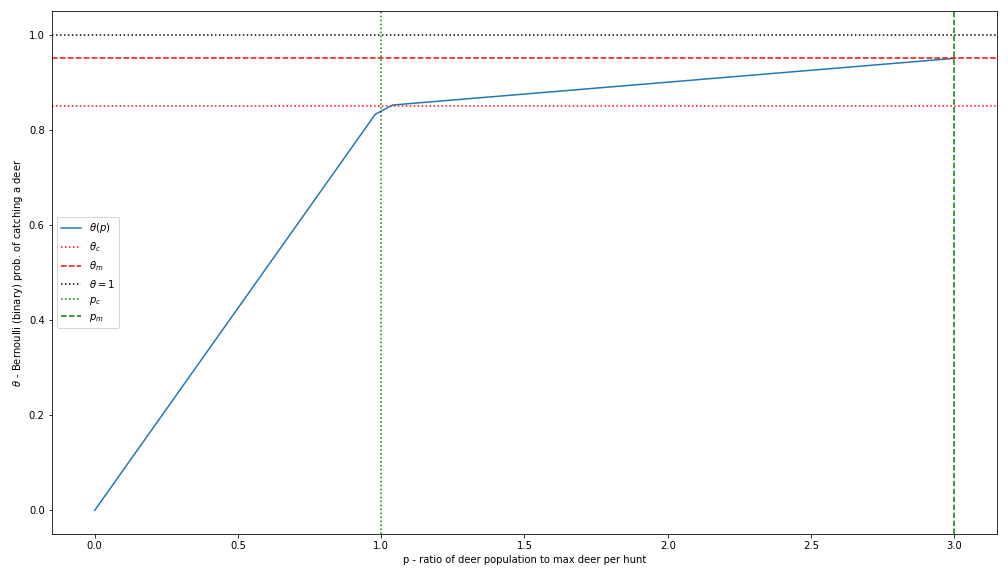
\includegraphics[width=1\textwidth]{04_environment/images/deer_pop_prob.png}
    \caption{Mapping function between the instantaneous deer population and the binary probability of catching a deer.}
    \label{fig:Foraging Mapping}
\end{figure}



\newpage
\section{Disasters}
\subsection{Disaster Background and type}

Table \ref{tab: Disaster's Main Function} contains a list of important functions accompanied by a functional and input/output description of each.

It is worth mentioning that an island's \texttt{geography} is the combination of the team ID and the island’s designated fixed location in the archipelago.

\begin{table}[!htb]
\begin{center}
\begin{tabular}{|l|l|l|l|l|}
\hline
\textbf{File}                                                                                 & \textbf{Function}                                                                        & \textbf{Description}                                                                                                                                               & \textbf{Inputs}                                                                                                             & \textbf{Outputs}                                                                                \\ \hline
\multirow{4}{*}{\texttt{\begin{tabular}[c]{@{}l@{}}environment\\ definition.go\end{tabular}}} & \texttt{\begin{tabular}[c]{@{}l@{}}Bernouilli\\ Distribution\\ (pdfGlobal)\end{tabular}} & \begin{tabular}[c]{@{}l@{}}Whether a \\ disaster \\ is going to \\ occur\end{tabular}                                                                              & \begin{tabular}[c]{@{}l@{}}- The probability of\\  a disaster occurring\\ - The Global \\ probability variable\end{tabular} & \begin{tabular}[c]{@{}l@{}}Determines the \\ likelyhoood of a \\ disaster occuring\end{tabular} \\ \cline{2-5} 
                                                                                              & \texttt{PdMag}                                                                           & \begin{tabular}[c]{@{}l@{}}Exponential\\ Distrubution\end{tabular}                                                                                                 & -  The spatial PDF                                                                                                          & \begin{tabular}[c]{@{}l@{}}Determine the \\ disaster \\ magnitude\end{tabular}                  \\ \cline{2-5} 
                                                                                              & \texttt{Epix, EpiY}                                                                      & \begin{tabular}[c]{@{}l@{}}Spatial \\ probability\\ distribution\\ function\end{tabular}                                                                           & \begin{tabular}[c]{@{}l@{}}- The spatial PDF\\ - Disaster \\ Magnitude\end{tabular}                                         & \begin{tabular}[c]{@{}l@{}}Determines the \\ location of the \\ disaster epicentre\end{tabular} \\ \cline{2-5} 
                                                                                              & \texttt{DisasterEffect}                                                                  & \begin{tabular}[c]{@{}l@{}}Island’s \\ Proximity\\ distance to the\\ eye of the storm\end{tabular}                                                                 & \begin{tabular}[c]{@{}l@{}}- Island geography\\ - Eye of the storm\\ location\end{tabular}                                  & \begin{tabular}[c]{@{}l@{}}Determine the \\ islands damag3\end{tabular}                         \\ \hline
\multirow{3}{*}{\texttt{Helpers.go}}                                                          & \texttt{island.X, island.Y}                                                              & Islands Georgraphy                                                                                                                                                 & - Island ID                                                                                                                 & \begin{tabular}[c]{@{}l@{}}- Islands fixed \\ position \\ coordinates\end{tabular}              \\ \cline{2-5} 
                                                                                              & \texttt{effects.Absolute}                                                                & \begin{tabular}[c]{@{}l@{}}Displays the total \\ disaster effects on \\ each islands\end{tabular}                                                                  & - Islands Geography                                                                                                         & individualEffect                                                                                \\ \cline{2-5} 
                                                                                              & \texttt{\begin{tabular}[c]{@{}l@{}}effects.\\ Proportional\end{tabular}}                 & \begin{tabular}[c]{@{}l@{}}Display proportional\\ disaster effects \\ relative to other \\ islands and effects \\ after the common \\ pool mitigation\end{tabular} & \begin{tabular}[c]{@{}l@{}}- Islands Geography\\ - Common Pool \\ Migiated resources\end{tabular}                           & proportionalEffect                                                                              \\ \hline
\end{tabular}
\end{center}
\caption{Disaster's Main Function}
\label{tab: Disaster's Main Function}
\end{table}

\subsection{Disaster Prevalence}
A disaster can be configured to occur with a with a \textbf{stochastic} or \textbf{deterministic} period \texttt{T} by toggling the \texttt{StochasticPeriod} parameter in the \texttt{DisasterConfig}.

These two cases are designed such that:
\begin{itemize}
    \item In the deterministic case, a disaster occurs regularly with a period $T_{0}$ (i.e. it is guaranteed to occur every $T$ turns).
    \item In the \texttt{stochastic} case, the expected period $E[T]$ = $T_0$.
\end{itemize}

Note that in the stochastic case, the period is a geometric random variable as it models the number of turns before a disaster strikes (assuming individual disaster samples on each turn are independent). If a disaster occurs on a given turn with probability $p$, the expected value of this geometric RV, the period, = $E[T]$ = $1/p$. In addition, since we want
$E[T]$ = $T_{0}$, $p$ is implied when $T_{0}$ is given. Therefore, only the period parameter has to be specified for both cases to be well defined.

\subsection {Disaster Severity and Location}

The magnitude and the location of disasters are sampled in from the same generating distributions for both types of periods.
The spatial (x, y) probability density function is configured by the \texttt{SpatialPDF} configuration parameter which defaults to \texttt{uniform}. This joint distribution is modelled as having two independent marginal x and y distributions and it controls the where the epicentre\footnote{location of peak magnitude} of a disaster occurs. The magnitude is exponentially distributed with a scale parameter \texttt{ExponentialRate} in the \texttt{DisasterConig}. Smaller exponential rate values result in a harsher environment and vice versa. This was chosen to model a plausible real life scenario where smaller disasters are far more common than very serious ones.
In addition, the disaster epicentre (`eye of the storm') is limited to the bounds of the environment which is predefined in the game configuration. When a disaster strikes, the effect (damage) felt by a given island is inversely proportional to the square of its distance to the epicentre of the disaster.

\begin{figure}[!htb]
    \centering
    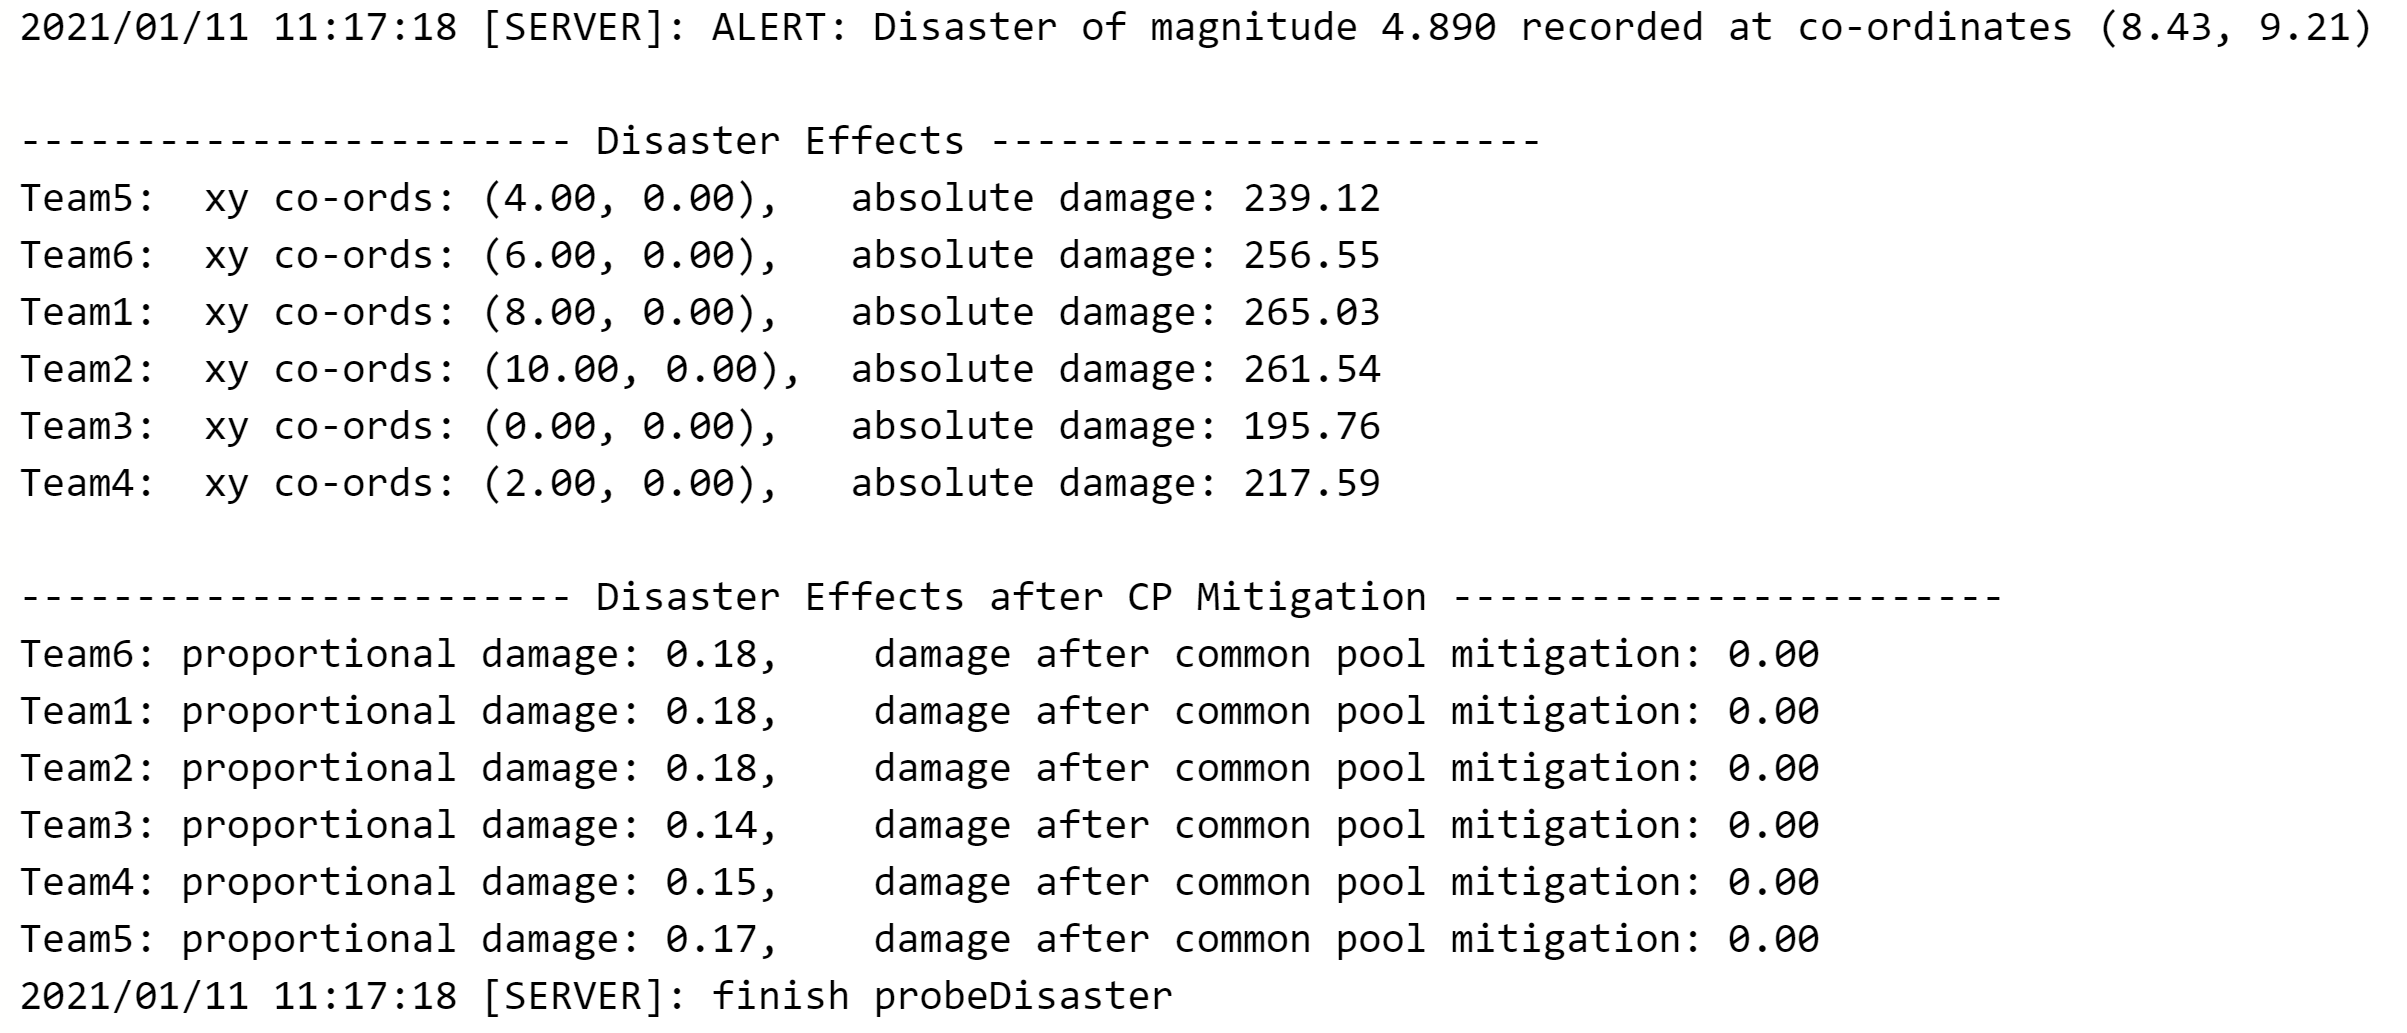
\includegraphics[width=1\textwidth]{04_environment/images/Disaster Effects Outcome.PNG}
    \caption{Infrastructure Disaster Effects outcome}
    \label{fig:Disaster Effects Outcome}
\end{figure}

Figure~\ref{fig:Disaster Effects Outcome} illustrates the output of the disaster. It shows the coordinates and peak magnitude of the disaster's epicentre, as well as the location of each island and the proportional effect on each island. For example, Island 1 located at (8,0) has the largest disaster effect due to its minimal proximity to the disaster epicentre of $265.03$.

\newpage
\section{Common Pool for Disaster Mitigation}

Table \ref{tab: Common Pool's Main Function} contains a list of important functions accompanied by a functional and input/output description of each.

\begin{table}[!htb]
%\vspace 1mm
\begin{center}
\begin{tabular}{|l|l|l|l|l|} 
\hline
\textbf{File}                                                                         & \textbf{Function}  & \textbf{Description}                                                                                                                                                & \textbf{Inputs}                                                                                                                                                                                                                 & \textbf{Outputs}                                                                                 \\ 
\hline
\multirow{4}{*}{\begin{tabular}[c]{@{}l@{}}environment\\ definition.go \end{tabular}} & IslandDistribute   & \begin{tabular}[c]{@{}l@{}}Distribute resources from \\Common~Pool to agents \\upon request\end{tabular}                                                            & \begin{tabular}[c]{@{}l@{}}- Requested resource\\amount\\ - island ID \end{tabular}                                                                                                                                             & None                                                                                             \\ 
\cline{2-5}
                                                                                      & IslandContribute   & \begin{tabular}[c]{@{}l@{}}Allows agents to \\contribute resources~\\towards Common Pool\end{tabular}                                                               & \begin{tabular}[c]{@{}l@{}}- Amount of resources\\to be contributed\\- Island ID \end{tabular}                                                                                                                                  & None                                                                                             \\ 
\cline{2-5}
                                                                                      & DisasterMitigate   & \begin{tabular}[c]{@{}l@{}}Computes the damage~\\mitigated by the CP and~\\the remaining damage~\\experienced by each\\island (if applicable)\end{tabular}          & \begin{tabular}[c]{@{}l@{}}- Effect of Disaster\\ to each island\\ - Proportional effect \\ of Disaster to each \\ island (magnitude \\ of disaster divided \\ by the distance of \\ the island from \\ epicenter \end{tabular} & \begin{tabular}[c]{@{}l@{}}Effects experiened by\\each island after CP\\mitigation\end{tabular}  \\ 
\cline{2-5}
                                                                                      & islandDeplete      & \begin{tabular}[c]{@{}l@{}}Deducts an amount of~\\resources from each\\island that is proportional\\to remaining disaster \\effect~after CP mitigation\end{tabular} & \begin{tabular}[c]{@{}l@{}}- Effects experiened by\\each island after CP\\mitigation\end{tabular}                                                                                                                               & None                                                                                             \\
\hline
\end{tabular}
\end{center}
\caption{Main functions of Common Pool for Disaster Mitigation}
\label{tab: Common Pool's Main Function}
\end{table}


This section details the implementation of Common Pool disaster mitigation. This includes a predetermined, constant \texttt{threshold} value that effectively represents a minimum required level of collective `insurance` against disasters. If a disaster occurs and the Common Pool resource level exceeds this threshold, the effects of the disaster are halved. If not, no such halving takes place and the full effect of the disaster is felt by the islands.

An important input to the implementation is the magnitude of the disaster’s damage on each island. In Figure~\ref{fig:Common Pool infrastructure outcome}, this specific disaster’s magnitude was 3.458. However, the disaster’s effect on individual islands does not add up to 3.458 because the storm’s epicenter is located some distance away from each island. This aspect creates a more realistic scenario. From the individual damage experienced by each island, proportional effects on each island are computed. The summation of these proportional effects is equal to 100$\%$, which is the total effective damage.\newline

When a disaster strikes the effect of the disaster on each islands is summed and compared to the resources in the common pool. If the common pool has more resources than the total effect of the disaster it can fully mitigate the disaster meaning the islands take not damage. However, in the unfortunate event that the total disaster damage exceeds Common Pool resources, the common is first depleted and the total disaster effect is also reduced by the same amount. Then, the remaining damage is applied to islands in proportion to the original damage they would have experienced (regardless of what their prior Common Pool contributions were). This is also visualised in Figure~\ref{fig:Common Pool infrastructure outcome}: Island 4 experiences the most damage from the storm and so, Island 4 receives the maximum Common Pool resource allocation of 252.47 resources (“common pool mitigated” column). The updated damage value shows the leftover damage of the disaster that the common pool was not able to mitigate. Left over damage serves to deplete an island's private pool of resources where applicable. If there is enough resources in the common pool to totally mitigate the disaster, the update damage values will be zero.

\begin{figure}[!htb]
    \centering
    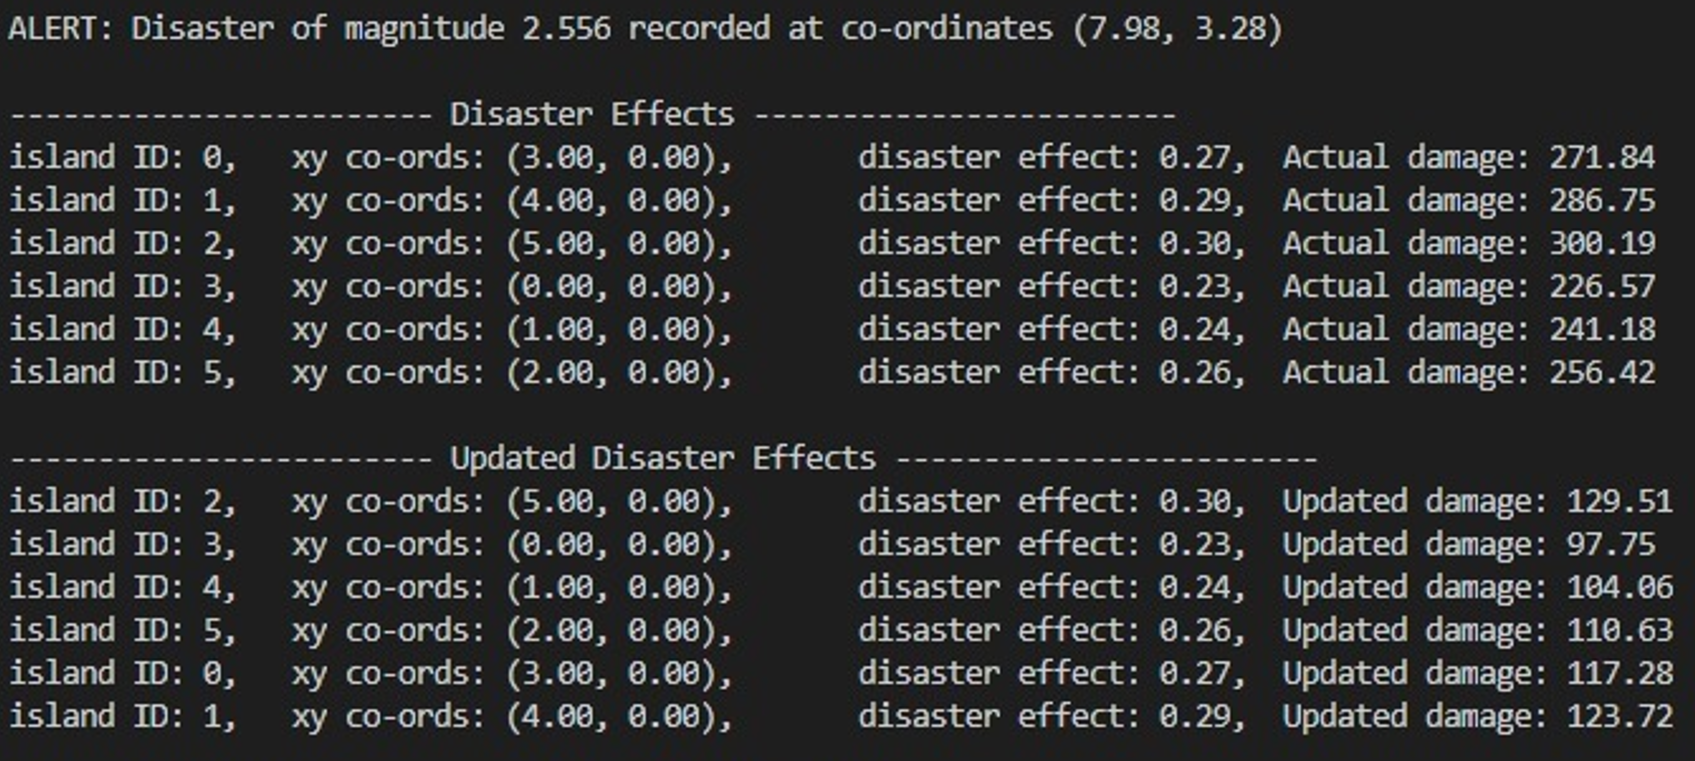
\includegraphics[width=1\textwidth]{04_environment/images/Common Pool infrastructure outcome.PNG}
    \caption{Demonstration of how common pool works in software}
    \label{fig:Common Pool infrastructure outcome}
\end{figure}

